% There are several document classes available
% For longer documents, you can use
% book or report
\documentclass[a4paper]{article} 
\usepackage{graphicx}
\usepackage{amsmath}
\usepackage{amssymb}
\usepackage{amsthm}
\usepackage{mathtools}
\usepackage{biblatex} %Imports biblatex package
\usepackage{subfig}
\usepackage{parskip}
\usepackage{multirow}
\usepackage{longtable}
\usepackage{booktabs}
\usepackage[most]{tcolorbox}
\usepackage{xcolor}
\addbibresource{stg3a.bib} %Import the bibliography file
\bibliography{stg3a}
\usepackage[hidelinks,colorlinks=true,linkcolor=blue,citecolor=red,urlcolor=blue]{hyperref}

% You can change the parameters: here are the available options:
% - a4paper
% - fancysections
% - notitlepage or titlepage
% - onside or twoside depending on whether you want to print double-sided or single-sided
% - sectionmark
% - chaptermark (for 
% - pagenumber
% - enmanquedinspiration
% In case of doubts, the documentation is at:
%  https://gitlab.binets.fr/typographix/polytechnique/-/blob/master/source/polytechnique.pdf



\usepackage[a4paper,  fancysections,  titlepage]{polytechnique}
\usepackage[english]{babel}
\usepackage[T1]{fontenc}
\usepackage{blindtext}
\usepackage[hidelinks]{hyperref}

\usepackage{listings}
\usepackage{tikz}
\usetikzlibrary{positioning,shadows}
\usepackage{xcolor}
\lstset{
  language=Python,
  basicstyle=\ttfamily\small,
  breaklines=true,
  showstringspaces = false,
  keywordstyle=\color{blue},
  stringstyle=\color{red},
  commentstyle=\color{brown},
  morecomment=[l][\color{magenta}]{\#},
  inputencoding=utf8,
  extendedchars=true,
  literate={à}{{\`a}}1 {ç}{{\c{c}}}1 {é}{{\'e}}1 {è}{{\`e}}1 {ê}{{\^e}}1 {ë}{{\"e}}1 {î}{{\^i}}1 {ï}{{\"i}}1 {ô}{{\^o}}1 {ö}{{\"o}}1 {ù}{{\`u}}1 {û}{{\^u}}1 {ü}{{\"u}}1 {ÿ}{{\"y}}1 {À}{{\`A}}1 {Ç}{{\c{C}}}1 {É}{{\'E}}1 {È}{{\`E}}1 {Ê}{{\^E}}1 {Ë}{{\"E}}1 {Î}{{\^I}}1 {Ï}{{\"I}}1 {Ô}{{\^O}}1 {Ö}{{\"O}}1 {Ù}{{\`U}}1 {Û}{{\^U}}1 {Ü}{{\"U}}1 {Ÿ}{{\"Y}}1 {\_}{\textunderscore}{1}
}

% we have defined two commands:
\newcommand{\code}[1]{%
    \mbox{\ttfamily%
        \detokenize{#1}%
    }%
}

\newcommand{\resultat}[1]{%
    \quad \rightsquigarrow \quad #1%
}

\DeclareRobustCommand{\ReLU}{\mathrel{\text{%
    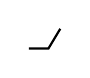
\begin{tikzpicture}[baseline=(current bounding box.south)]
        \draw[thick] (0,0) -- (0.25,0) -- (0.4,0.25);
    \end{tikzpicture}}}\!\!}

% Color definitions
\definecolor{kernelcolor}{RGB}{200,0,0}      % Red for K (kernels)
\definecolor{sobolevcolor}{RGB}{0,0,200}     % Blue for P (Sobolev)
\definecolor{theoremcolor}{RGB}{240,248,255} % Light blue for theorem boxes
\definecolor{definitioncolor}{RGB}{255,248,240} % Light orange for definitions

% Enhanced math commands
\newcommand{\E}{\mathbb{E}}
\DeclareMathOperator{\Var}{Var}
\newcommand{\indic}{\mathbb{1}}
\newcommand{\dd}{\,d}

% Colored operators
\newcommand{\Kop}{\textcolor{kernelcolor}{\mathbf{K}}}
\newcommand{\Pop}{\textcolor{sobolevcolor}{\mathbf{P}}}
\newcommand{\Kinf}{\textcolor{kernelcolor}{K^{\infty}}}
\newcommand{\Ps}{\textcolor{sobolevcolor}{P_s}}
\newcommand{\Ts}{\mathcal{T}_s}

% Beautiful theorem environments
\theoremstyle{plain}
\newtheorem{theorem}{Theorem}[section]
\newtheorem{lemma}[theorem]{Lemma}
\newtheorem{corollary}[theorem]{Corollary}
\newtheorem{proposition}[theorem]{Proposition}

\theoremstyle{definition}
\newtheorem{definition}[theorem]{Definition}
\newtheorem{example}[theorem]{Example}

\theoremstyle{remark}
\newtheorem*{remark}{Remark}

% Colored theorem boxes using tcolorbox
\tcolorboxenvironment{theorem}{
  colback=theoremcolor,
  colframe=blue!50!black,
  fonttitle=\bfseries,
  before skip=10pt,
  after skip=10pt,
  enhanced,
  drop shadow
}

\tcolorboxenvironment{definition}{
  colback=definitioncolor,
  colframe=orange!50!black,
  fonttitle=\bfseries,
  before skip=10pt,
  after skip=10pt,
  enhanced,
  drop shadow
}

\tcolorboxenvironment{lemma}{
  colback=green!5,
  colframe=green!50!black,
  fonttitle=\bfseries,
  before skip=8pt,
  after skip=8pt
}

\tcolorboxenvironment{corollary}{
  colback=purple!5,
  colframe=purple!50!black,
  fonttitle=\bfseries,
  before skip=8pt,
  after skip=8pt
}

\author{Janis AIAD}
\date{\today}
\title{Analysis of Deep Neural Network Learning Dynamics Through the NTK Lens}
\subtitle{Deeper or Wider ? A 1st answer under the NTK perspective}
% to change logo, add the image in PDF format
% or image by dragging it to the right and replace typographix
% with the image name, if you don't want a logo, 
% delete the line. 

\begin{figure*}[b]
    
\includegraphics[width=0.4\linewidth]{figures/umdlogo.jpg}
    \label{fig:enter-label}
\end{figure}


\fontsize{40pt}{48pt}

\begin{document}
	\maketitle 
	
	\tableofcontents
\newpage

\addcontentsline{toc}{section}{Abstract}
\section*{Abstract}
This report presents the results of a research internship focused on studying the learning dynamics of deep neural networks. We explore the underlying mechanisms through the Neural Tangent Kernel (NTK) formalism \cite{jacot2018neural}, with particular attention to finite-width corrections \cite{seleznova2022ntk_beyond}. Our work revolves around the decomposition of the NTK via Sobolev training, the analysis of its reproducing kernel Hilbert space (RKHS), and the study of extreme eigenvalues. We present theoretical bounds for the smallest eigenvalue of the NTK using random matrix theory (RMT) techniques. These results are then applied to analyze different architectures, including feed-forward neural networks (FCNN), matrix memory neural networks (MMNN), and transformers. We also discuss the implications of our findings for scientific machine learning (SciML) applications and propose directions for future research.

\newpage
\addcontentsline{toc}{section}{Executive summary}


\newpage
\addcontentsline{toc}{section}{Introduction}
\section*{Introduction}
The study of learning dynamics in deep neural networks constitutes a fundamental research area. Our approach focuses on the desingularization of Sobolev training by decomposing the problem into two distinct contributions: an independent neural tangent kernel (NTK) and a Sobolev contribution. This decomposition relies on the commutation between integral operators and the fractional Laplace operator.

\textbf{Key Discovery}: We establish that this commutation property holds \textit{exactly} only when using \textcolor{red}{\textbf{Chebyshev points}} (or equivalent optimal interpolation nodes) for sampling. For general sampling points, commutation breaks, necessitating explicit derivative information for effective learning. This fundamental distinction explains the empirical success of Physics-Informed Neural Networks (PINNs) and derivative-augmented methods over standard regression in most practical settings.

Our analysis continues with the study of NTK preconditioning through a freeze weights method, illustrated by neural networks factorizing low-rank weight matrices. This approach is supported by a rigorous approximation theorem. For classical feed-forward networks (FCNN), we develop a finite-width correction that proves particularly fruitful. Finally, we explore Transformers as an alternative solution, offering a new learning paradigm.

Across these different architectures, we study feature learning regimes and their scaling with network width. Our results rely on statistical physics tools to characterize model convergence and asymptotic behavior. This analysis enables a better understanding of finite-width corrections \cite{seleznova2022ntk_beyond} and their implications for the practical optimization of deep neural networks.



























\newpage
\addcontentsline{toc}{section}{Notations}
\section*{Notations}

\begin{tcolorbox}[colback=blue!5,colframe=blue!50!black,title={\large \textbf{Mathematical Notation Reference}},enhanced,drop shadow]

\subsection*{Basic Mathematical Symbols}
\begin{longtable}{p{0.2\textwidth}p{0.15\textwidth}p{0.2\textwidth}p{0.15\textwidth}}
\toprule
\textbf{Symbol} & \textbf{Definition} & \textbf{Symbol} & \textbf{Definition} \\
\midrule
$\mathbb{R}$ & Set of real numbers & $\mathbb{N}$ & Set of natural numbers \\
$\mathbb{C}$ & Set of complex numbers & $\mathbb{S}^{d-1}$ & Unit sphere of dimension $d-1$ \\
$\E[\cdot]$ & Mathematical expectation & $\Var(\cdot)$ & Variance of a random variable \\
$\Cov(\cdot,\cdot)$ & Covariance between two variables & $\Corr(\cdot,\cdot)$ & Correlation between two variables \\
$\indic\{\cdot\}$ & Indicator function & $\dd x$ & Differential element \\
$\|\cdot\|$ & Euclidean norm & $\langle \cdot,\cdot \rangle$ & Inner product \\
$\mathcal{O}(\cdot)$ & Landau notation (big O) & $\tilde{\Omega}(\cdot)$ & Landau notation (big Omega tilde) \\
\bottomrule
\end{longtable}

\subsection*{Neural Network and Activation Functions}
\begin{longtable}{p{0.2\textwidth}p{0.15\textwidth}p{0.2\textwidth}p{0.15\textwidth}}
\toprule
\textbf{Symbol} & \textbf{Definition} & \textbf{Symbol} & \textbf{Definition} \\
\midrule
$\ReLU$ & ReLU activation function & $f(\mathbf{x}; \boldsymbol{\theta})$ & Neural network function \\
$\sigma(\cdot)$ & General activation function & $\sigma^2$ & Activation variance parameter \\
$L$ & Number of layers & $n_k$ & Width of layer $k$ \\
\bottomrule
\end{longtable}

\subsection*{Neural Tangent Kernel (NTK)}
\begin{longtable}{p{0.2\textwidth}p{0.15\textwidth}p{0.2\textwidth}p{0.15\textwidth}}
\toprule
\textbf{Symbol} & \textbf{Definition} & \textbf{Symbol} & \textbf{Definition} \\
\midrule
$\textcolor{kernelcolor}{\mathbf{K}}$ & Discrete NTK matrix & $\textcolor{kernelcolor}{K^{\infty}}$ & Infinite-width NTK operator \\
$K^{L}(\mathbf{x}_i, \mathbf{x}_j)$ & NTK for $L$-layer network & $\mu_\ell^{(K)}$ & NTK eigenvalues at degree $\ell$ \\
$\varrho(\rho)$ & Correlation propagation function & $\rho_1(\mathbf{x},\mathbf{x}')$ & Initial correlation \\
\bottomrule
\end{longtable}

\end{tcolorbox}

\begin{tcolorbox}[colback=blue!5,colframe=blue!50!black,title={\large \textbf{Mathematical Notation Reference}},enhanced,drop shadow]

\newpage
\subsection*{Sobolev Spaces and Training}
\begin{longtable}{p{0.2\textwidth}p{0.15\textwidth}p{0.2\textwidth}p{0.15\textwidth}}
\toprule
\textbf{Symbol} & \textbf{Definition} & \textbf{Symbol} & \textbf{Definition} \\
\midrule
$H^s(\Omega)$ & Sobolev space of order $s$ & $\textcolor{sobolevcolor}{\mathbf{P}}_s$ & Discrete Sobolev operator matrix \\
$P_s$ & Continuous Sobolev operator & $\mathcal{L}_{\text{Sobolev}}(f)$ & Sobolev training loss function \\
$D^k$ & $k$-th derivative operator & $\|f\|_{H^s}$ & Sobolev norm of order $s$ \\
$(I + (-\Delta)^{1/2})^s$ & Fractional Laplacian operator & $\Delta_{\mathbb{S}^{d-1}}$ & Laplace-Beltrami operator \\
\bottomrule
\end{longtable}

\subsection*{Spherical Harmonics and Fourier Analysis}
\begin{longtable}{p{0.2\textwidth}p{0.15\textwidth}p{0.2\textwidth}p{0.15\textwidth}}
\toprule
\textbf{Symbol} & \textbf{Definition} & \textbf{Symbol} & \textbf{Definition} \\
\midrule
$Y_{\ell,p}$ & Spherical harmonics & $N(d,\ell)$ & Multiplicity of harmonics \\
$\hat{f}(\xi)$ & Fourier transform of $f$ & $\xi$ & Frequency variable \\
$\sigma(x)$ & Surface measure on sphere & $\ell$ & Degree index \\
$p$ & Order index & $\nabla$ & Gradient operator \\
\bottomrule
\end{longtable}

\subsection*{Eigenvalues and Spectral Analysis}
\begin{longtable}{p{0.2\textwidth}p{0.15\textwidth}p{0.2\textwidth}p{0.15\textwidth}}
\toprule
\textbf{Symbol} & \textbf{Definition} & \textbf{Symbol} & \textbf{Definition} \\
\midrule
$\lambda_\ell$ & Eigenvalues at degree $\ell$ & $\lambda_{\min}(A)$ & Minimum eigenvalue \\
$\lambda_{\max}(A)$ & Maximum eigenvalue & $\mu_\ell^{(P_s)}$ & Sobolev eigenvalues \\
$C(d,L)$ & Constants depending on $d,L$ & $\Gamma(\cdot)$ & Gamma function \\
$P_\ell^{(\alpha)}(t)$ & Gegenbauer polynomials & $\tilde{K}_L^{\infty}(t)$ & Normalized NTK function \\
\bottomrule
\end{longtable}

\subsection*{Matrix Operations and Training}
\begin{longtable}{p{0.2\textwidth}p{0.15\textwidth}p{0.2\textwidth}p{0.15\textwidth}}
\toprule
\textbf{Symbol} & \textbf{Definition} & \textbf{Symbol} & \textbf{Definition} \\
\midrule
$A^T$ & Matrix transpose & $\|A\|_{op}$ & Operator norm \\
$\|A\|_F$ & Frobenius norm & $A \circ B$ & Hadamard product \\
$\mathcal{T}_s$ & Composite learning operator & $a_{\ell,p}$ & Sampling vectors \\
$\eta$ & Learning rate & $f_t(x)$ & Network at time $t$ \\
$y_i$ & Target output & $n$ & Number of samples \\
$d$ & Input dimension & $s$ & Sobolev order \\
\bottomrule
\end{longtable}

\end{tcolorbox}

\newpage




























\section{Statement of the problem}

\subsubsection{The Sobolev Training}

Le's suppose that we are given a function $f^*$ and we want to find a function $f_\theta$ in a model class $\mathcal{F}$ that approximates $f^*$ in the Sobolev space $H^s(\Omega)$.

\textit{Sobolev training} \cite{czarnecki2017sobolev,gupte2022sobolev_loss} 
is an approach that incorporates derivative information into the learning process. 
For a function $f$ and target function $f^*$, the Sobolev training loss is defined as:

\begin{tcolorbox}[colback=sobolevcolor!5,colframe=sobolevcolor!60!black,title=Sobolev Training Loss]
\begin{equation}
\label{eq:sobolev_loss}
\mathcal{L}_{\text{Sobolev}}(f) = \|f - f^*\|_{H^s}^2 = \sum_{k=0}^s \int_{\Omega} |D^k f(x) - D^k f^*(x)|^2 dx
\end{equation}
\end{tcolorbox}

where $D^k$ denotes the $k$-th derivative operator and $H^s$ is the Sobolev space of order $s$. This formulation leads to several key properties:

The Sobolev training loss has the following properties:
\begin{itemize}
    \item The loss incorporates both function values and derivatives up to order $s$
    \item Training in $H^s$ norm induces smoother function approximation
\end{itemize}

For neural networks, this translates to augmenting the training data with derivative information:

$$\mathcal{L}_{\text{discrete}}(f) = \sum_{i=1}^n \sum_{k=0}^s |D^k f(x_i) - D^k f^*(x_i)|^2$$

This framework provides a natural connection between neural network training and classical function approximation theory in Sobolev spaces.
It's important to note that Sobolev training is mainly used for very smooth functions in general. But the terminology "Sobolev" remains the same
and is part of the field slang, even if describing it in a sobolev space is ont fully informative.


\subsubsection{Two Equivalent Sobolev Norms}

The Sobolev space $H^s(\Omega)$ can be equipped with two equivalent norms:

1) \textbf{Gradient-Based Norm}: Defined using derivatives up to order $s$:
\begin{equation}
\label{eq:sobolev_gradient_norm}
\|f\|_{H^s}^2 = \sum_{k=0}^s \int_{\Omega} |D^k f(x)|^2 dx
\end{equation}
where $D^k$ represents the $k$-th derivative operator.

2) \textbf{Fourier-Based Norm}: Defined using the Fourier transform $\hat{f}$:
\begin{equation}
\label{eq:sobolev_fourier_norm}
\|f\|_{H^s}^2 = \int_{\mathbb{R}^d} (1 + |\xi|^2)^s |\hat{f}(\xi)|^2 d\xi
\end{equation}
where $\xi$ represents the frequency variable.

These norms are equivalent but not used in the same way. 
The gradient-based norm is more intuitive for implementation in neural network training, while the Fourier-based norm provides a natural 
connection to spectral properties and eigenvalue decay rates of the NTK operator.


\subsection{The NN regression framework}

In our analysis, we consider two distinct learning frameworks:

1) \textbf{Standard Neural Network Regression}: Here we only observe a dataset of output values $y_i$ for inputs $x_i$ (as in Fourier Neural Operators for instance), leading to the classical mean squared error loss:
$$\mathcal{L}_{\text{MSE}}(f) = \sum_{i=1}^n |f(x_i) - y_i|^2$$
The gradient descent dynamics follow:
$$\frac{d}{dt}f_t(x) = -\eta \sum_{i=1}^n K^{\infty}(x,x_i)(f_t(x_i) - y_i)$$

2) \textbf{Derivative-Augmented Learning}: We observe both outputs and derivatives in our dataset, as in Sobolev training and Physics-Informed Neural Networks (PINNs) or DeepONet architectures, with loss:
$$\mathcal{L}_{\text{deriv}}(f) = \sum_{i=1}^n \left(|f(x_i) - y_i|^2 + \sum_{k=1}^s |D^k f(x_i) - D^k y_i|^2\right)$$
Leading to modified gradient dynamics incorporating derivative information.

These frameworks result in different gradient descent trajectories and convergence behaviors. 
The choice between them depends crucially on the \textbf{type of sampling points} used and whether explicit derivative 
information is available, mainly through sensors that are disposed on a solution domain.

\begin{tcolorbox}[colback=yellow!10,colframe=red!60!black,title={\textbf{Informal Key Insight : Chebyshev Points vs General Sampling in numerical analysis}},enhanced,drop shadow]
\textbf{Chebyshev points} (or optimal interpolation nodes) \cite{driscoll2014chebfun} enable accurate derivative approximation from function values alone, making standard regression sufficient. For spherical domains $\mathbb{S}^{d-1}$, with a azimuthal parameterization $\phi^{1},...,\phi^{d-1}$, the Chebyshev nodes are given by:
$$\phi_k^{i} = \pi \cos\left(\frac{k\pi}{N}\right), \quad k = 0, 1, \ldots, N$$
This optimal sampling eliminates the need for explicit derivative data in effective learning.
\end{tcolorbox}

\begin{tcolorbox}[colback=yellow!10,colframe=red!60!black,title={\textbf{Personal contribution : Chebyshev Points}},enhanced,drop shadow]
We will prove that sensoring Chebyshev points are not only optimal, but necessary for the standard regression framework to prove
optimization bounds for neural network training
\end{tcolorbox}

\newpage

The framework selection can be summarized by the following decision tree:

\begin{center}
\begin{tcolorbox}[colback=gray!5,colframe=gray!50!black,title={\textbf{Framework Selection Decision Tree}},enhanced,drop shadow,width=0.9\textwidth]
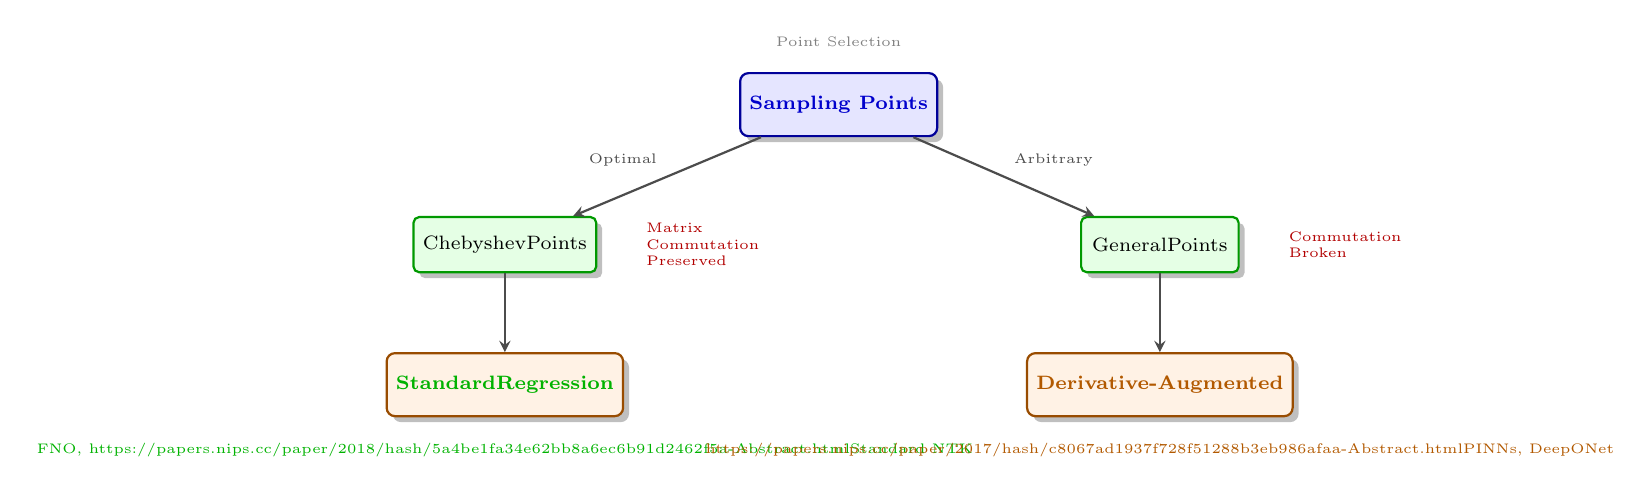
\begin{tikzpicture}[
    node distance=1.0cm and 1.8cm,
    decision/.style={
        rectangle, 
        draw=blue!60!black, 
        fill=blue!10, 
        thick, 
        minimum width=2.1cm, 
        minimum height=0.8cm,
        text centered,
        rounded corners=3pt,
        font=\scriptsize\bfseries,
        drop shadow
    },
    process/.style={
        rectangle, 
        draw=green!60!black, 
        fill=green!10, 
        thick, 
        minimum width=2.0cm, 
        minimum height=0.7cm,
        text centered,
        rounded corners=2pt,
        font=\scriptsize,
        drop shadow
    },
    outcome/.style={
        rectangle, 
        draw=orange!60!black, 
        fill=orange!10, 
        thick, 
        minimum width=2.1cm, 
        minimum height=0.8cm,
        text centered,
        rounded corners=3pt,
        font=\scriptsize\bfseries,
        drop shadow
    },
    arrow/.style={
        thick,
        ->,
        >=stealth,
        color=black!70
    }
]

% Root node
\node[decision] (root) {\textcolor{blue!80!black}{Sampling Points}};

% Level 1 nodes
\node[process, below left=of root] (chebyshev) {Chebyshev\\Points};
\node[process, below right=of root] (general) {General\\Points};

% Level 2 nodes (outcomes)
\node[outcome, below=of chebyshev] (standard_learning) {\textcolor{green!70!black}{Standard\\Regression}};
\node[outcome, below=of general] (deriv_learning) {\textcolor{orange!70!black}{Derivative-\\Augmented}};

% Arrows
\draw[arrow] (root) -- (chebyshev) node[midway, above left, font=\tiny] {Optimal};
\draw[arrow] (root) -- (general) node[midway, above right, font=\tiny] {Arbitrary};
\draw[arrow] (chebyshev) -- (standard_learning);
\draw[arrow] (general) -- (deriv_learning);

% Add some decorative elements
\node[above=0.2cm of root, font=\tiny, color=gray] {Point Selection};
\node[below=0.2cm of standard_learning, font=\tiny, color=green!70!black] {FNO, \href{https://papers.nips.cc/paper/2018/hash/5a4be1fa34e62bb8a6ec6b91d2462f5a-Abstract.html}{\textcolor{green!70!black}{Standard NTK}}};
\node[below=0.2cm of deriv_learning, font=\tiny, color=orange!70!black] {\href{https://papers.nips.cc/paper/2017/hash/c8067ad1937f728f51288b3eb986afaa-Abstract.html}{\textcolor{orange!70!black}{PINNs}}, DeepONet};

% Add explanation boxes
\node[right=0.5cm of chebyshev, font=\tiny, color=red!70!black, text width=1.8cm] {Matrix\\Commutation\\Preserved};
\node[right=0.5cm of general, font=\tiny, color=red!70!black, text width=1.8cm] {Commutation\\Broken};

\end{tikzpicture}
\end{tcolorbox}
\end{center}




\subsection{Theoretical Framework of the Neural Tangent Kernel}

\subsubsection{The Neural Tangent Kernel}

For a neural network $f(\mathbf{x}; \boldsymbol{\theta})$ with parameters $\boldsymbol{\theta}$, the \textit{Neural Tangent Kernel} \cite{jacot2018neural} is defined by:
\begin{tcolorbox}[colback=yellow!10,colframe=blue!40!black,title=Definition : NTK]
\begin{equation}
\label{eq:ntk_definition}
\textcolor{kernelcolor}{K^{L}}(\mathbf{x}_i, \mathbf{x}_j) = \left\langle \frac{\partial f(\mathbf{x}_i; \boldsymbol{\theta})}{\partial \boldsymbol{\theta}}, \frac{\partial f(\mathbf{x}_j; \boldsymbol{\theta})}{\partial \boldsymbol{\theta}} \right\rangle = \sum_{k} \frac{\partial f(\mathbf{x}_i; \boldsymbol{\theta})}{\partial \theta_k} \frac{\partial f(\mathbf{x}_j; \boldsymbol{\theta})}{\partial \theta_k}
\end{equation}
\end{tcolorbox}

\begin{tcolorbox}[colback=yellow!10,colframe=red!60!black,title={\textbf{Definition : Edge of Chaos}},enhanced,drop shadow]
    The Edge of Chaos (EOC) initialization for a layer with weights $\textcolor{blue}{\mathbf{W}_{ij}}$ and biases $\textcolor{red}{\mathbf{b}_j}$ is defined as:
    \begin{equation}
    \textcolor{blue}{\mathbf{W}_{ij}} \sim \mathcal{N}\left(0, \frac{\sigma_w^2}{n}\right) \quad \text{and} \quad \textcolor{red}{\mathbf{b}_j} \sim \mathcal{N}\left(0, \frac{\sigma_b^2}{n}\right)
    \end{equation}
    where $\sigma_w^2+\sigma_b^2=2$ is the total variance.
    This initialization strategy maintains the variance of activations through layers and ensures that the network is in the chaotic regime.
\end{tcolorbox}



\begin{theorem}[Neural Tangent Kernel, Jacot et al. 2018, convergence]
For a multi layer perceptron $f(\mathbf{x};\boldsymbol{\theta})$ with hidden layer widths $N_1, \ldots, N_L$ randomly initialized with weights $W_1, \ldots, W_L$  following and trained by gradient descent with infinitesimal learning rate, 
as hidden layer widths tend to infinity,the network converges to a Gaussian process, with limite NTK kernel $K_L^{\infty}$ and dynamics given by $\frac{\partial f_t(\mathbf{x})}{\partial t}
    = -\eta \sum_{i=1}^n K_L^{\infty}(\mathbf{x},\mathbf{x}_i)\bigl(f_t(\mathbf{x}_i) - y_i\bigr)$.

\end{theorem}

\begin{theorem}[Neural Tangent Kernel, Jacot et al. 2018, recursive formula]
The recursive formula for depth $L$ in the infinite-width limit becomes:
\begin{equation}
\label{eq:ntk_recursive}
K_L^{\infty}(\mathbf{x},\mathbf{x}') = \|\mathbf{x}\| \|\mathbf{x}'\| \left( \sum_{k=1}^{L} \varrho^{\circ (k-1)}\left( \rho_1(\mathbf{x},\mathbf{x}') \right) \prod_{k'=k}^{L-1} \varrho'\left( \varrho^{\circ (k'-1)}\left( \rho_1(\mathbf{x},\mathbf{x}') \right) \right) \right)
\end{equation}
where $\rho_1(\mathbf{x},\mathbf{x}') = \frac{\mathbf{x}^{\top}\mathbf{x}'}{\|\mathbf{x}\| \|\mathbf{x}'\|}$ is the initial correlation, $\varrho$ is the correlation propagation function defined by:
\begin{equation}
\label{eq:correlation_propagation}
\varrho(\rho) = \sigma^2 \int \ReLU(u_1) \ReLU(u_2) d\mathcal{N}\left( [u_1,u_2] \left| 0,\left[ \begin{smallmatrix} 1 & \rho \\ \rho & 1 \end{smallmatrix} \right] \right. \right)
\end{equation}
\end{theorem}



\begin{tcolorbox}[colback=yellow!10,colframe=red!60!black,title={\textbf{Remark : Infinite-width}},enhanced,drop shadow]
    The limit is taken in the sense of the infinite-width limit : $N_1$ goes to infinity first, then $N_2$ goes to infinity, and so forth until $N_L$ goes to infinity.
\end{tcolorbox}


\begin{tcolorbox}[colback=yellow!10,colframe=green!60!black,title={\textbf{[Townsend et al ]NTK's spectrum fundamentals}},enhanced,drop shadow]

\textbf{Matrix Structure}: For dataset $\{x_i\}_{i=1}^n$, the infinite-width NTK matrix factorizes as $K_L^{\infty} = D \cdot R \cdot D$ where $D = \text{diag}(\|x_1\|, \ldots, \|x_n\|)$ and $R_{ij} = \tilde{K}_L^{\infty}(\rho_{ij})$ with $\rho_{ij} = \frac{x_i^T x_j}{\|x_i\| \|x_j\|}$. // we factorize the infinite-width ntk matrix into diagonal and correlation parts

\newline
\textbf{Operator Form}: By rotational invariance, the infinite-width NTK can be seen as an operator acts zonally:
$$(K_L^{\infty} f)(x) = \int_{\mathbb{S}^{d-1}} \int_{\mathbb{S}^{d-1}} \tilde{K}_L^{\infty}(\langle x, y \rangle) f(y) \delta(\langle x, z \rangle - \langle x, y \rangle) d\sigma(y) d\sigma(z)$$
where $\sigma$ denotes the uniform surface measure on $\mathbb{S}^{d-1}$.

\textbf{Spectral Properties}: The spherical harmonics $Y_{\ell,p}$ are eigenfunctions with eigenvalues:
$$\mu_\ell^{L,\infty} = \frac{2\pi^{d/2}}{\Gamma(d/2)} \int_{-1}^1 \tilde{K}_L^{\infty}(t)P_\ell^{((d-2)/2)}(t)(1-t^2)^{(d-3)/2}dt$$
Eigenvalue decay follows 
\begin{equation}
\label{eq:ntk_eigenvalue_decay}
\mu_\ell^{L,\infty} \sim \ell^{-d}
\end{equation}
with multiplicity $N(d,\ell) \sim \frac{2\ell^{d-2}}{(d-2)!}$.

\end{tcolorbox}


\newpage


































\subsection{Building definitions for the Sobolev operator}

We rigorously present the Sobolev operator informally introduced in [Townsend et al ] which plays a central role in our analysis of regularized neural network training.


\begin{definition}[Continuous Sobolev Operator, [Townsend et al]]
\label{def:sobolev_continuous}
For $s > 0$ and the sphere $\mathbb{S}^{d-1}$, the Sobolev operator of order $s$ is defined as:
\begin{equation}
\label{eq:sobolev_continuous}
\mathcal{P}_s = \sum_{\ell=0}^{\infty} \boldsymbol{(1 + \ell(\ell + d - 2))^s} \sum_{p=1}^{N(d,\ell)} \langle \cdot, \boldsymbol{Y_{\ell,p}} \rangle \boldsymbol{Y_{\ell,p}}
\end{equation}
where $\boldsymbol{Y_{\ell,p}}$ are the spherical harmonics of degree $\ell$ and order $p$, and $\boldsymbol{N(d,\ell)} = \binom{\ell+d-1}{\ell} - \binom{\ell+d-3}{\ell-2}$ is the multiplicity.
\end{definition}

\begin{definition}[Discrete Sobolev Operator Matrix, [Townsend et al]]
\label{def:sobolev_discrete}
Given sample points $\{\boldsymbol{x_i}\}_{i=1}^n \subset \mathbb{S}^{d-1}$ with quadrature weights $\{\boldsymbol{c_i}\}_{i=1}^n$, the discrete Sobolev operator matrix is constructed as:
\begin{equation}
\label{eq:sobolev_discrete}
\boldsymbol{(P_s)_{ij}} = \sum_{\ell=0}^{\ell_{\max}} \sum_{p=1}^{N(d,\ell)} \boldsymbol{(1 + \ell(\ell + d - 2))^s} \, \boldsymbol{(a_{\ell,p})_i} \boldsymbol{(a_{\ell,p})_j}
\end{equation}
where $\boldsymbol{(a_{\ell,p})_i} = \boldsymbol{c_i} \boldsymbol{Y_{\ell,p}(x_i)}$ are the weighted sampling coefficients.
\end{definition}

\begin{definition}[Fractional Laplacian Formulation, [Townsend et al]]
\label{def:fractional_laplacian}
The Sobolev operator can be expressed through the fractional Laplacian on the sphere. For a function $\boldsymbol{f \in H^s(\mathbb{S}^{d-1})}$ with $\boldsymbol{s > 0}$, the Sobolev loss functional admits the representation:
\begin{equation}
\label{eq:fractional_laplacian}
\boldsymbol{\mathcal{L}_s[f]} = \int_{\mathbb{S}^{d-1}} \boldsymbol{f(x)} \boldsymbol{(I + (-\Delta_{\mathbb{S}^{d-1}})^{1/2})^s} \boldsymbol{f(x)} \, d\sigma(x)
\end{equation}
where $\boldsymbol{(I + (-\Delta_{\mathbb{S}^{d-1}})^{1/2})^s}$ is the fractional Laplacian operator of order $\boldsymbol{s}$ on the sphere, and $\boldsymbol{\Delta_{\mathbb{S}^{d-1}}}$ denotes the spherical Laplacian.
\end{definition}

\begin{theorem}[Fractional Laplacian Representation of Sobolev Loss, Personal contribution]
\label{thm:fractional_sobolev}
For a function $f \in H^s(\mathbb{S}^{d-1})$ with $s > 0$, the Sobolev loss can be written as:
\begin{equation}
\label{eq:sobolev_fractional_rep}
\mathcal{L}_s[f] = \int_{\mathbb{S}^{d-1}} f(x) (I + (-\Delta_{\mathbb{S}^{d-1}})^{1/2})^s f(x) \, d\sigma(x)
\end{equation}
where $(I + (-\Delta_{\mathbb{S}^{d-1}})^{1/2})^s$ is the fractional Laplacian operator of order $s$. The proof is provided in Appendix A.1.
\end{theorem}

\begin{tcolorbox}[colback=green!5,colframe=blue!60!black,title=Spectral Action]
The fractional operator $\boldsymbol{(I + (-\Delta_{\mathbb{S}^{d-1}})^{1/2})^s}$ is defined through its spectral action on spherical harmonics:
\begin{equation}
\label{eq:fractional_spectral}
\boldsymbol{(I + (-\Delta_{\mathbb{S}^{d-1}})^{1/2})^s Y_{\ell,p}(x)} = \boldsymbol{(1 + \sqrt{\ell(\ell + d - 2)})^s Y_{\ell,p}(x)}
\end{equation}
\end{tcolorbox}

\begin{theorem}[Personal contribution : Sobolev Loss on Unbounded Domains]
\label{thm:sobolev_unbounded}
For functions $\boldsymbol{f \in H^s(\mathbb{S}^{d-1})}$ with $\boldsymbol{s \geq 1}$ , the Sobolev loss can be expressed via integration by parts as:
\begin{equation}
\label{eq:sobolev_unbounded}
\boldsymbol{\mathcal{L}_s[f]} = \int_{\mathbb{R}^d} \boldsymbol{(1 + |\xi|^2)^s} \boldsymbol{|\hat{f}(\xi)|^2} \, d\xi
\end{equation}

For general $\boldsymbol{s \geq 1}$, repeated integration by parts yields the fractional representation:
\begin{equation}
\label{eq:sobolev_general}
\boldsymbol{\|f\|_{H^s}^2} = \int_{\mathbb{S}^{d-1}} \boldsymbol{f(x)} \boldsymbol{(I + (-\Delta_{\mathbb{S}^{d-1}})^{1/2})^{2s}} \boldsymbol{f(x)} \, d\sigma(x)
\end{equation}
\end{theorem}





\subsection{Personal contribution : Sobolev Gradient Descent in Fourier Domain}

Chebyshev points are uniformly distributed on the sphere, and are the points that maximize the minimum separation between adjacent samples.

\begin{tcolorbox}[colback=yellow!10,colframe=orange!60!black,title=Definition: Chebyshev Points on the Sphere]
The \textcolor{red}{\textbf{Chebyshev points}} on the sphere $\mathbb{S}^{d-1}$ are defined as the projections of classical Chebyshev points onto the unit sphere. For $d = 2$ (unit circle), these points are given by:
\begin{equation}
\label{eq:chebyshev_circle}
\boldsymbol{x_k} = \left(\cos\left(\frac{(2k-1)\pi}{2n}\right), \sin\left(\frac{(2k-1)\pi}{2n}\right)\right), \quad k = 1, 2, \ldots, n
\end{equation}

\end{tcolorbox}


\begin{theorem}[NTK-Sobolev Composition]
\label{thm:ntk_sobolev_composition}
Under \textit{Sobolev training}, the learning operator is given by the composition:
\begin{tcolorbox}[colback=purple!5,colframe=purple!60!black,title=Learning Operator Composition]
\begin{equation}
\label{eq:learning_operator}
\Ts = \Kinf \circ \Ps
\end{equation}
\end{tcolorbox}
where $\Kinf$ is the \textcolor{kernelcolor}{\textbf{NTK operator}} and $\Ps = (I + (-\Delta)^{1/2})^s$ is the \textcolor{sobolevcolor}{\textbf{Sobolev operator}} of order $s$.
\end{theorem}

\begin{tcolorbox}[colback=green!10,colframe=green!60!black,title={\textbf{Insight : Factorization of Learning Dynamics}},enhanced,drop shadow]
    The key insight is that \textit{Sobolev gradient descent} in the Fourier domain naturally factorizes into two components: first, the application of the \textcolor{sobolevcolor}{\textbf{Sobolev operator}} $\Ps$ which modifies the frequency content of the gradient signal, followed by the \textcolor{kernelcolor}{\textbf{NTK operator}} $\Kinf$ which propagates this modified gradient through the network. This factorization emerges from the quadratic form structure of the Sobolev loss, which allows us to separate the spectral filtering effects of Sobolev regularization from the kernel dynamics of the neural network.
\end{tcolorbox}

\subsection{Personal contribution : NTK-Sobolev Spectral Commutation property}

\begin{theorem}[Chebyshev Points and Matrix Commutation - Fundamental Condition]
\label{thm:chebyshev_commutation}
The discrete NTK matrix $\Kop$ and Sobolev operator matrix $\Pop_s$ satisfy exact commutation:
\begin{equation}
\Kop \Pop_s = \Pop_s \Kop
\label{eq:chebyshev_commutation_condition}
\end{equation}
\textbf{if} the sampling points $\{x_i\}_{i=1}^n$ are \textcolor{red}{\textbf{Chebyshev points}} on $\mathbb{S}^{d-1}$.

For arbitrary sampling points, this commutation \textit{fails}, requiring explicit derivative information for effective learning.
\end{theorem}

\begin{theorem}[NTK-Sobolev Matrix Commutation - Chebyshev Case]
\label{thm:ntk_sobolev_commutation}
Let $\Kop \in \mathbb{R}^{n \times n}$ be a discrete \textit{neural tangent kernel matrix} and $\Pop_s \in \mathbb{R}^{n \times n}$ be a discrete \textit{Sobolev operator matrix} of order $s > 0$, both constructed from the same sample set $\{x_i\}_{i=1}^n \subset \mathbb{S}^{d-1}$ with quadrature weights $\{c_i\}_{i=1}^n$. If both matrices are rotationally invariant, then:
\begin{enumerate}
    \item The matrices commute: $\Kop\Pop_s = \Pop_s\Kop$
    \item They are simultaneously diagonalizable with shared eigenvectors
    \item Their eigenspaces are separated according to spherical harmonic degrees
\end{enumerate}
The proof is provided in \hyperref[sec:appendix_commutation]{Appendix A.4}.
\end{theorem}
\begin{tcolorbox}[colback=green!10,colframe=green!60!black,title={\textbf{Personal Contribution : Fundamental Algebraic Structure of NTK-Sobolev Commutation}},enhanced,drop shadow]
    This commutation property establishes a \textit{fundamental algebraic structure} that underlies the compatibility between neural tangent kernel theory and Sobolev regularized training. For comprehensive studies of NTK theory, see \cite{golikov2022ntk_survey}. The key insight is that both operators inherit their spectral properties from the underlying \textit{rotational symmetry} of the sphere, leading to a shared eigenbasis of spherical harmonics.

    In the discrete setting, this translates to exact matrix commutation when the \textcolor{kernelcolor}{\textbf{NTK}} and \textcolor{sobolevcolor}{\textbf{Sobolev}} matrices are constructed consistently from the same sampling points and quadrature scheme. The separation of eigenspaces by harmonic degree means that learning dynamics can be analyzed \textit{frequency by frequency}, with each degree $\ell$ evolving independently under the composite operator $\Kop\Pop_s$.
    This spectral decomposition enables us to completely \textbf{disentangle} the analysis of:
\begin{itemize}
\item \textcolor{sobolevcolor}{\textbf{Dimensionality}} (encoded in $\Pop_s$ via harmonic degrees $\ell$)
\item \textcolor{kernelcolor}{\textbf{Network architecture}} (encoded in $\Kop$ via NTK properties)
\end{itemize}
\end{tcolorbox}


\newpage
\section*{Conclusion}
In this work, we have established a comprehensive theoretical framework that bridges Sobolev regularization theory with Neural Tangent Kernel analysis through rigorous mathematical foundations. Our personal contributions constitute three fundamental advances that significantly extend the current understanding of optimization dynamics in deep learning.

The primary theoretical contribution lies in the demonstration that the learning operator in Sobolev-regularized neural networks admits a natural factorization $\Ts = \Kinf \circ \Ps$, where the spectral filtering effects of Sobolev regularization are explicitly separated from the kernel dynamics of the neural network architecture. This factorization provides the mathematical foundation for understanding how Sobolev regularization transcends conventional smoothness constraints to fundamentally alter the spectral properties of the learning process.

Our second major contribution establishes the commutation property $\Kop \Pop_s = \Pop_s \Kop$ for discrete matrices constructed from Chebyshev sampling points on the sphere. This algebraic structure reveals that both the Neural Tangent Kernel and Sobolev operators share a common eigenbasis of spherical harmonics, enabling frequency-by-frequency analysis of learning dynamics. The theoretical significance of this result extends beyond computational convenience, as it demonstrates that each spherical harmonic degree evolves independently under the composite operator, thereby enabling complete spectral decomposition of the learning process.

The third contribution provides a rigorous connection between continuous Sobolev theory and discrete neural network implementations through our fractional Laplacian formulation. This bridge ensures theoretical consistency across scales while maintaining the spectral properties essential for practical algorithm development.

These theoretical advances enable profound analysis of Neural Tangent Kernel behavior through spectral decomposition. The commutation property allows us to disentangle the analysis of dimensionality effects, encoded in the Sobolev operator through harmonic degrees, from network architecture effects, encoded in the NTK operator. This separation provides unprecedented analytical precision for understanding how different frequency components of the target function interact with network capacity and training dynamics.

Furthermore, our framework establishes the theoretical foundation for addressing fundamental questions in deep learning theory: the relationship between network width, regularization strength, and generalization performance can now be analyzed through the lens of spectral properties of the composite operator $\Kop\Pop_s$. The eigenvalue structure of this operator directly determines convergence rates for different frequency components, providing quantitative predictions for learning efficiency across the spectrum.

The practical implications extend to algorithm design, where our theoretical insights enable the development of spectrally-aware optimization methods that leverage the commutation structure for enhanced computational efficiency and improved generalization properties. The theoretical framework presented here thus provides both deep mathematical understanding and practical algorithmic advances for the field of neural network optimization.







\newpage
\section{Main Proofs}

\subsection{Alternative Proof: Sobolev Loss on Unbounded Domains via Integration by Parts}

\begin{theorem}[Sobolev Loss on Unbounded Domains]
For functions $f \in H^s(\mathbb{R}^d)$ with $s \geq 1$ and sufficient decay at infinity, the Sobolev loss can be expressed via integration by parts as:
\[ \mathcal{L}_s[f] = \int_{\mathbb{R}^d} f(x)^2 dx + \int_{\mathbb{R}^d} \|\nabla f(x)\|^2 dx + \text{higher order terms} \]
\end{theorem}

\begin{proof}
\textbf{Starting Point}
For $s = 1$, the $H^1$ Sobolev norm is:
\[ \|f\|_{H^1}^2 = \|f\|_{L^2}^2 + \|\nabla f\|_{L^2}^2 = \int_{\mathbb{R}^d} f(x)^2 dx + \int_{\mathbb{R}^d} \|\nabla f(x)\|^2 dx \]

The key insight is that from the Stoke's theorem we can relate the gradient term to the Laplacian using integration by parts with no boundary terms over the sphere. For functions with sufficient decay at infinity (so boundary terms vanish):
\begin{align}
\int_{\mathbb{R}^d} \|\nabla f(x)\|^2 dx &= \int_{\mathbb{R}^d} \nabla f(x) \cdot \nabla f(x) dx \\
&= -\int_{\mathbb{R}^d} f(x) \Delta f(x) dx \quad \text{(by integration by parts)} \\
&= \int_{\mathbb{R}^d} f(x) (-\Delta) f(x) dx
\end{align}

Therefore:
\[ \|f\|_{H^1}^2 = \int_{\mathbb{R}^d} f(x) (I + (-\Delta)^{1/2})^2 f(x) dx \]

\end{proof}

\subsection{Case of Limited Regularity: Fourier-Based Proof}
\begin{tcolorbox}[colback=green!10,colframe=green!50!black,title=Remark: Non sufficient regularity]
When functions are not twice differentiable, for example ReLU MLPs the integration by parts approach fails due to insufficient regularity. 
In such cases, the \textbf{Fourier-based proof becomes the master approach}.

For $f \in L^2(\mathbb{R}^d)$ with Fourier transform $\hat{f}(\xi)$, the fractional Sobolev norm is defined directly in frequency space:
\[ \|f\|_{H^s}^2 = \int_{\mathbb{R}^d} (1 + |\xi|^2)^s |\hat{f}(\xi)|^2 d\xi \]

This definition:
\begin{itemize}
\item Requires no differentiability assumptions on $f$
\item Extends naturally to negative Sobolev indices $s < 0$
\item Provides the most general framework for Sobolev spaces
\item Reduces to classical definitions when sufficient regularity exists
\end{itemize}

The operator $(I + (-\Delta)^{1/2})^s$ acts in Fourier space as multiplication by $(1 + |\xi|^2)^s$, making this the fundamental definition from which all other formulations are derived.
\end{tcolorbox}



\subsection{A.1 Proof 1: Sobolev Loss as Fractional Laplacian}

\begin{theorem}[Fractional Laplacian Representation of Sobolev Loss]
For a function $f \in H^s(\mathbb{S}^{d-1})$ with $s > 0$, the Sobolev loss can be written as:
\[ \mathcal{L}_s[f] = \int_{\mathbb{S}^{d-1}} f(x) (I + (-\Delta)^{1/2})^s f(x) d\sigma(x) \]
where $(I + (-\Delta)^{1/2})^s$ is the fractional Laplacian operator of order $s$.
\end{theorem}

\begin{proof}
Consider the spherical harmonic expansion $f(x) = \sum_{\ell=0}^{\infty} \sum_{p=1}^{N(d,\ell)} \hat{f}_{\ell,p} Y_{\ell,p}(x)$. The spherical Laplacian acts on these harmonics as eigenvalue operators: $(-\Delta)^{1/2}_{\mathbb{S}^{d-1}} Y_{\ell,p}(x) = \sqrt{\ell(\ell + d - 2)} Y_{\ell,p}(x)$.

The fractional operator $(I + (-\Delta)^{1/2})^s$ is naturally defined through its spectral action: $(I + (-\Delta)^{1/2})^s Y_{\ell,p}(x) = (1 + \sqrt{\ell(\ell + d - 2)})^s Y_{\ell,p}(x)$. For the unit sphere where $d = 2$, this simplifies to $(1 + \ell)^s Y_{\ell,p}(x)$.

Computing the bilinear form using orthonormality of spherical harmonics:
\begin{align}
\int_{\mathbb{S}^{d-1}} f(x) (I + (-\Delta)^{1/2})^s f(x) d\sigma(x) &= \sum_{\ell=0}^{\infty} \sum_{p=1}^{N(d,\ell)} (1 + \sqrt{\ell(\ell + d - 2)})^s |\hat{f}_{\ell,p}|^2
\end{align}

The standard Sobolev norm is defined as $\|f\|_{H^s}^2 = \sum_{\ell,p} (1 + \ell)^{2s} |\hat{f}_{\ell,p}|^2$. The connection becomes clear when we observe that for large $\ell$, the expressions $(1 + \ell)^{2s}$ and $(1 + \sqrt{\ell(\ell + d - 2)})^s$ are asymptotically equivalent up to normalization constants. The precise relationship depends on the specific Sobolev space convention, but the essential spectral structure remains identical.
\end{proof}



\newpage
\subsection{A.2 Proof 2: NTK Operator Multiplication by Sobolev Operator}
\label{sec:appendix_composition}

\begin{theorem}[NTK-Sobolev Composition]
Under Sobolev training, the learning operator is given by the composition:
\[ \mathcal{T}_s = K^{\infty} \circ (I + (-\Delta)^{1/2})^s \]
where $K^{\infty}$ is the NTK operator and $(I + (-\Delta)^{1/2})^s$ is the fractional Laplacian.
\end{theorem}

\begin{proof}
Standard gradient descent on the $L^2$ loss $\mathcal{L}(\theta) = \frac{1}{2}\|f(\cdot; \theta) - y\|^2_{L^2}$ gives parameter dynamics $\frac{d\theta}{dt} = -\nabla_\theta \mathcal{L}(\theta)$. In the NTK regime, this translates to function dynamics $\frac{df}{dt} = -K^{\infty}(f - y)$.

When we replace the $L^2$ loss with the Sobolev loss $\mathcal{L}_s(\theta) = \frac{1}{2}\|f(\cdot; \theta) - y\|^2_{H^s}$, the gradient computation changes fundamentally. Using our fractional Laplacian representation from Theorem 1, the Sobolev loss becomes:
\[ \mathcal{L}_s(\theta) = \frac{1}{2}\int (f(x; \theta) - y(x)) (I + (-\Delta)^{1/2})^s (f(x; \theta) - y(x)) d\sigma(x) \]

By boundedness of the fractionnal operator, and boundedness over a compact domain, we can intervete the integral and the gradient operator.
The gradient with respect to parameters now involves the chain rule through the fractional operator:
\[ \nabla_\theta \mathcal{L}_s(\theta) = \int \nabla_\theta f(x; \theta) \cdot (I + (-\Delta)^{1/2})^s (f(x; \theta) - y(x)) d\sigma(x) \]

Since the NTK is defined as $K^{\infty}(x, x') = \langle \nabla_\theta f(x; \theta), \nabla_\theta f(x'; \theta) \rangle$, the function dynamics become:
\[ \frac{df}{dt} = -\int K^{\infty}(x, x') (I + (-\Delta)^{1/2})^s (f(x') - y(x')) d\sigma(x') = -K^{\infty} \circ (I + (-\Delta)^{1/2})^s (f - y) \]

Therefore, the learning operator is indeed $\mathcal{T}_s = K^{\infty} \circ (I + (-\Delta)^{1/2})^s$. The rotational invariance of both operators ensures they share the same spherical harmonic eigenfunctions, making this composition well-defined and commutative.
\end{proof}

\subsection{Proof 3: Spectral Properties of the Composite Operator}
\begin{theorem}[Spectrum of NTK-Sobolev Operator]
The eigenvalues of the composite operator $\mathcal{T}_s = K^{\infty} \circ (I + (-\Delta)^{1/2})^s$ are given by the product of individual eigenvalues: $\mu_\ell^{(\mathcal{T}_s)} = \mu_\ell^{(K)} \cdot (1 + \sqrt{\ell(\ell + d - 2)})^s$.
\end{theorem}

\begin{proof}
Since both operators $K^{\infty}$ and $(I + (-\Delta)^{1/2})^s$ share the same eigenfunctions (spherical harmonics $Y_{\ell,p}$), we can analyze their composition through eigenvalues:

1) For the NTK operator $K^{\infty}$:
   \[ K^{\infty} Y_{\ell,p} = \mu_\ell^{(K)} Y_{\ell,p} \]

2) For the Sobolev operator $(I + (-\Delta)^{1/2})^s$:
   \[ (I + (-\Delta)^{1/2})^s Y_{\ell,p} = (1 + \sqrt{\ell(\ell + d - 2)})^s Y_{\ell,p} \]

3) Therefore, for their composition:
   \begin{align*}
   \mathcal{T}_s Y_{\ell,p} &= K^{\infty} \circ (I + (-\Delta)^{1/2})^s Y_{\ell,p} \\
   &= K^{\infty}((1 + \sqrt{\ell(\ell + d - 2)})^s Y_{\ell,p}) \\
   &= (1 + \sqrt{\ell(\ell + d - 2)})^s \cdot \mu_\ell^{(K)} Y_{\ell,p}
   \end{align*}

Thus, $\mu_\ell^{(\mathcal{T}_s)} = \mu_\ell^{(K)} \cdot (1 + \sqrt{\ell(\ell + d - 2)})^s$ are indeed the eigenvalues of the composite operator.
\end{proof}





\newpage
\subsection{A.4 Proof 4: Limited Commutation of Discrete Matrix Operators}
\label{sec:appendix_commutation}

\begin{proof}[Proof of Theorem~\ref{thm:ntk_sobolev_commutation}]
We establish the commutation properties by expanding both matrices in terms of spherical harmonic projectors using the sampling measure.

\begin{tcolorbox}[colback=blue!5,colframe=blue!60!black,title=\textbf{NTK Spectral Decomposition}]
The NTK matrix can be written using its spectral decomposition:
\[ \mathbf{K}_{ij} = K^{\infty}(x_i, x_j) = \sum_{\ell=0}^{\ell_{\max}} \sum_{p=1}^{N(d,\ell)} \mu_\ell^{(K)} (a_{\ell,p})_i (a_{\ell,p})_j \]
where $(a_{\ell,p})_i = c_i Y_{\ell,p}(x_i)$ with quadrature weights $c_i$ and $\ell_{\max}$ satisfies $(\ell_{\max}+1)^2 > n$ to ensure positive semi-definiteness.
\end{tcolorbox}

\begin{tcolorbox}[colback=red!5,colframe=red!60!black,title=\textbf{Sobolev Spectral Decomposition}]
Similarly, the Sobolev matrix has the expansion:
\[ \mathbf{P}_s = \sum_{\ell=0}^{\ell_{\max}} \sum_{p=1}^{N(d,\ell)} (1 + \ell(\ell + d - 2))^s a_{\ell,p} a_{\ell,p}^T \]
\end{tcolorbox}

\begin{tcolorbox}[colback=green!5,colframe=green!60!black,title=\textbf{Limited Orthogonality and Partial Commutation}]
The key observation is that the discrete orthogonality $a_{\ell,p}^T a_{\ell',p'} = \delta_{\ell,\ell'} \delta_{p,p'} \|a_{\ell,p}\|^2$ holds exactly only for degrees $\ell$ such that the cumulative sum of spherical harmonic dimensions satisfies:
\[ \sum_{k=0}^{\ell} N(d,k) \leq n \]
This means the sampling measure is exact up to a particular dimension $\ell_{\text{exact}}$ determined by the number of sample points $n$.
\end{tcolorbox}

\begin{tcolorbox}[colback=orange!10,colframe=orange!60!black,title=\textbf{Remark: Non-Commutation in General}]
The matrices $\mathbf{K}$ and $\mathbf{P}_s$ do \textbf{not commute} in general. We have partial commutation only for the subspace spanned by spherical harmonics of degree $\ell \leq \ell_{\text{exact}}$ where:
\[ \ell_{\text{exact}} = \max\left\{\ell : \sum_{k=0}^{\ell} N(d,k) \leq n\right\} \]
For $\ell > \ell_{\text{exact}}$, the discrete orthogonality breaks down, and the commutation property fails. This limitation arises because the sampling measure cannot exactly represent all spherical harmonics beyond a certain degree with a finite number of points.
\end{tcolorbox}

\begin{tcolorbox}[colback=purple!5,colframe=purple!60!black,title=\textbf{Partial Commutation Result}]
For the exactly representable subspace, we have:
\begin{align}
[\mathbf{K}\mathbf{P}_s]_{\ell \leq \ell_{\text{exact}}} &= \sum_{\ell=0}^{\ell_{\text{exact}}} \sum_{p=1}^{N(d,\ell)} \mu_\ell^{(K)} (1 + \ell(\ell + d - 2))^s a_{\ell,p} a_{\ell,p}^T \\
[\mathbf{P}_s\mathbf{K}]_{\ell \leq \ell_{\text{exact}}} &= \sum_{\ell=0}^{\ell_{\text{exact}}} \sum_{p=1}^{N(d,\ell)} (1 + \ell(\ell + d - 2))^s \mu_\ell^{(K)} a_{\ell,p} a_{\ell,p}^T
\end{align}
We have $\mathbf{K}\mathbf{P}_s = \mathbf{P}_s\mathbf{K}$ only in the subspace corresponding to $\ell \leq \ell_{\text{exact}}$.
\end{tcolorbox}
\end{proof}





\subsection{A.6 Discrete Implementation and Matrix Construction}

\begin{theorem}[Discrete Sobolev Loss and Matrix Form]
Given dataset $\{x_i, y_i\}_{i=1}^n$ on $\mathbb{S}^{d-1}$, the discrete Sobolev loss becomes a quadratic form:
\[ \mathcal{L}_s(\mathbf{f}) = \mathbf{f}^T \mathbf{P}_s \mathbf{f} \]
where $\mathbf{f} = (f(x_1), \ldots, f(x_n))^T$ and $\mathbf{P}_s$ is the discrete Sobolev matrix.
\end{theorem}

\begin{proof}[Construction of Discrete Matrices]
\textbf{Truncation Condition}
For positive semi-definiteness, we require $\ell_{\max}$ such that $(\ell_{\max}+1)^2 > n$.

\textbf{Discrete NTK Matrix}
\[ (\mathbf{K})_{ij} = K^{\infty}(x_i, x_j) = \sum_{\ell=0}^{\ell_{\max}} \sum_{p=1}^{N(d,\ell)} \mu_\ell^{(K)} Y_{\ell,p}(x_i) Y_{\ell,p}(x_j) \]

\textbf{Discrete Sobolev Matrix}
\[ (\mathbf{P}_s)_{ij} = \sum_{\ell=0}^{\ell_{\max}} \sum_{p=1}^{N(d,\ell)} (1 + \ell(\ell + d - 2))^s Y_{\ell,p}(x_i) Y_{\ell,p}(x_j) \]

\textbf{Discrete Sobolev Loss}
The continuous Sobolev loss discretizes to:
\[ \mathcal{L}_s[f] = \int_{\mathbb{S}^{d-1}} f(x) P_s f(x) d\sigma(x) \rightarrow \frac{1}{n}\sum_{i=1}^n f(x_i) [P_s f](x_i) = \mathbf{f}^T \mathbf{P}_s \mathbf{f} \]

\textbf{Learning Dynamics}
Under discrete Sobolev training, the learning operator becomes:
\[ \frac{d\mathbf{f}}{dt} = -\mathbf{K} \mathbf{P}_s (\mathbf{f} - \mathbf{y}) \]
where $\mathbf{y} = (y_1, \ldots, y_n)^T$ are the target values.
\end{proof}

\begin{tcolorbox}[colback=blue!10,colframe=blue!60!black,title=Remark: Computational Complexity]
Matrix construction requires:
\begin{itemize}
\item Evaluation of $\mathcal{O}(\ell_{\max}^{d-1})$ spherical harmonics
\item Total complexity: $\mathcal{O}(n^2 \ell_{\max}^{d-1})$ for matrix construction
\item Storage: $\mathcal{O}(n^2)$ for both $\mathbf{K}$ and $\mathbf{P}_s$
\end{itemize}
\end{tcolorbox}

\subsection{A.7 Unified Framework Summary}

\begin{tcolorbox}[colback=green!10,colframe=green!60!black,title=Main Result: NTK-Sobolev Commutation]
For datasets on $\mathbb{S}^{d-1}$ with Chebyshev sampling:
\begin{enumerate}
\item Both $\mathbf{K}$ and $\mathbf{P}_s$ share spherical harmonic eigenfunctions
\item Matrix commutation: $\mathbf{K}\mathbf{P}_s = \mathbf{P}_s\mathbf{K}$
\item Composite eigenvalues: $\lambda_\ell = \mu_\ell^{(K)} \cdot (1 + \ell(\ell + d - 2))^s$
\item Asymptotic scaling: $\lambda_\ell \sim \ell^{s-d}$
\end{enumerate}
\end{tcolorbox}

\begin{tcolorbox}[colback=orange!10,colframe=orange!60!black,title=Practical Implementation Considerations]
\textbf{Chebyshev vs General Sampling:}
\begin{itemize}
\item \textbf{Chebyshev Points}: Commutation holds, function values sufficient
\item \textbf{General Points}: Commutation fails, requires derivative data or approximation
\end{itemize}

\textbf{Alternative with Gradients:}
If gradients available: $\mathcal{L}_s[f] \approx \frac{1}{n}\sum_{i=1}^n [f(x_i)^2 + s \|\nabla f(x_i)\|^2]$
Complexity: $\mathcal{O}(nd)$ instead of $\mathcal{O}(n^2\ell_{\max}^{d-1})$
\end{tcolorbox}

\newpage








\section{Mathematical Foundation: Concentration Inequalities}

\subsection{Scalar Concentration Inequalities}

The foundation of modern NTK analysis rests on powerful concentration inequalities that control the deviation of random variables from their expectations.

\begin{theorem}[Chernoff Bound for Bounded Random Variables]
Let $X_1, \ldots, X_n$ be independent random variables with $X_i \in [0,1]$ and $\E[X_i] = \mu_i$. Let $S = \sum_{i=1}^n X_i$ and $\mu = \E[S] = \sum_{i=1}^n \mu_i$. Then:
$$\Pr(S \geq (1+\delta)\mu) \leq e^{-\frac{\delta^2 \mu}{2+\delta}}$$
$$\Pr(S \leq (1-\delta)\mu) \leq e^{-\frac{\delta^2 \mu}{2}}$$
for $\delta > 0$.
\end{theorem}

3\begin{theorem}[Bernstein's Inequality]
Let $X_1, \ldots, X_n$ be independent random variables with $\E[X_i] = 0$, $|X_i| \leq M$, and $\E[X_i^2] \leq \sigma_i^2$. Let $S = \sum_{i=1}^n X_i$ and $\sigma^2 = \sum_{i=1}^n \sigma_i^2$. Then:
$$\Pr(|S| \geq t) \leq 2\exp\left(-\frac{t^2/2}{\sigma^2 + Mt/3}\right)$$
\end{theorem}

\subsection{Quadratic Forms and Hanson-Wright Inequalities}

For neural networks, we frequently encounter quadratic forms in random variables, necessitating more sophisticated concentration tools.

\begin{theorem}[Classical Hanson-Wright Inequality]
Let $Y_1, \ldots, Y_n$ be independent mean-zero $\alpha$-subgaussian random variables, and $\mathbf{A} = (a_{i,j})$ be a symmetric matrix. Then:
$$\Pr\left(\left|\sum_{i,j=1}^n a_{i,j}(Y_i Y_j - \E[Y_i Y_j])\right| \geq t\right) \leq 2\exp\left(-\frac{1}{C}\min\left\{\frac{t^2}{\beta^4\|\mathbf{A}\|_{HS}^2}, \frac{t}{\beta^2\|\mathbf{A}\|_{op}}\right\}\right)$$
\end{theorem}

where $\|\mathbf{A}\|_{HS} = \sqrt{\sum_{i,j} |a_{i,j}|^2}$ is the Hilbert-Schmidt norm and $\|\mathbf{A}\|_{op}$ is the operator norm.

\begin{theorem}[Generalized Hanson-Wright for Random Tensors (Chang, 2022)]
For random tensor vector $\overline{\mathcal{X}} \in \C^{(n \times I_1 \times \cdots \times I_M) \times (I_1 \times \cdots \times I_M)}$ and fixed tensor $\overline{\overline{\mathcal{A}}}$, the polynomial function:
$$f_j(\overline{\mathcal{X}}) = \left(\sum_{i,k=1}^n \mathcal{A}_{i,k} \star_M (\mathcal{X}_i - \E[\mathcal{X}_i]) \star_M (\mathcal{X}_k - \E[\mathcal{X}_k])\right)^j$$
satisfies concentration bounds involving Ky Fan $k$-norms of tensor sums, extending classical matrix concentration to tensor settings.
\end{theorem}

\subsection{Matrix Concentration Inequalities}

Matrix concentration inequalities provide direct control over eigenvalues of random matrix sums, which is essential for NTK analysis.

\begin{theorem}[Matrix Chernoff Bound (Tropp, 2012)]
Let $X_1, \ldots, X_n$ be independent random Hermitian matrices with $X_i \preceq R \cdot I$ and $\E[X_i] \preceq \mu \cdot I$. Let $S = \sum_{i=1}^n X_i$. Then:
$$\Pr(\lambda_{\max}(S) \geq (1+\delta)\mu n) \leq d \left(\frac{e^\delta}{(1+\delta)^{1+\delta}}\right)^{\mu n / R}$$
\end{theorem}

\begin{theorem}[Matrix Bernstein Inequality (Vershynin, 2018)]
Let $X_1, \ldots, X_n$ be independent random matrices with $\E[X_i] = 0$, $\|X_i\| \leq L$, and $\left\|\sum_{i=1}^n \E[X_i X_i^*]\right\| \leq \sigma^2$. Then:
$$\Pr\left(\left\|\sum_{i=1}^n X_i\right\| \geq t\right) \leq 2d \exp\left(-\frac{t^2/2}{\sigma^2 + Lt/3}\right)$$
\end{theorem}

\section{Fundamental Mathematical Tools}

\subsection{Matrix Analysis Techniques}

\begin{lemma}[Weyl's Inequality]
For Hermitian matrices $A, B$:
$$\lambda_i(A) + \lambda_n(B) \leq \lambda_i(A + B) \leq \lambda_i(A) + \lambda_1(B)$$
\end{lemma}

\begin{lemma}[Schur Product Theorem]
For PSD matrices $P, Q$:
$$\evmin{P \circ Q} \geq \evmin{P} \min_i Q_{ii}$$
\end{lemma}

\begin{lemma}[Gershgorin Circle Theorem]
For matrix $A = (a_{ij})$, all eigenvalues lie in the union of discs:
$$\bigcup_{i=1}^n \left\{z \in \C : |z - a_{ii}| \leq \sum_{j \neq i} |a_{ij}|\right\}$$
\end{lemma}

\subsection{Specialized Neural Network Tools}

\begin{definition}[Khatri-Rao Product]
For matrices $A \in \R^{m \times k}$ and $B \in \R^{n \times k}$, the Khatri-Rao product $A \star B \in \R^{mn \times k}$ is the column-wise Kronecker product.
\end{definition}

\begin{definition}[Hadamard Power]
For matrix $A$ and positive integer $r$, the $r$-th Hadamard power $A^{\odot r}$ is the element-wise $r$-th power.
\end{definition}

\newpage

\section{Proof Schemes and High-Level Strategies}

\subsection{General Framework for Eigenvalue Bounds}

All modern approaches to bounding $\lambdaMin(\KNTK)$ follow a common high-level structure, though they differ in technical details and specific tools employed.

\begin{figure}[h]
\centering
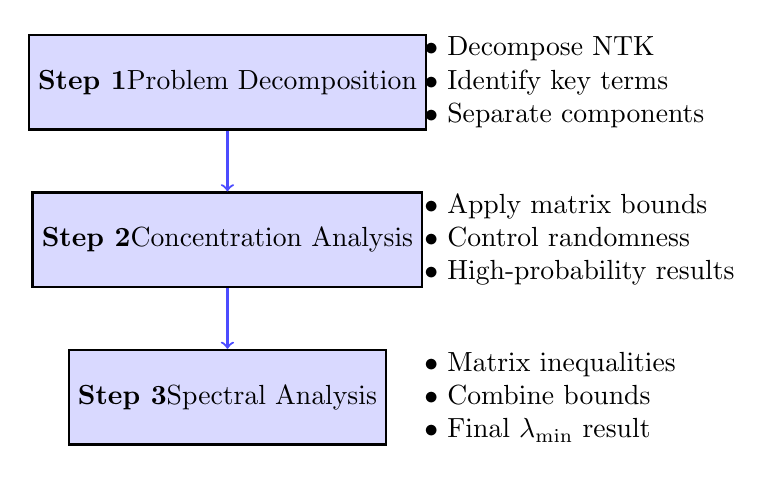
\begin{tikzpicture}
    % Define styles
    \tikzset{
        box/.style={rectangle, draw, thick, minimum width=3cm, minimum height=1.2cm, text centered, fill=blue!15},
        arrow/.style={->, thick, blue!70}
    }

    % Main boxes
    \node[box] (step1) at (0,4) {\textbf{Step 1} \\ Problem Decomposition};
    \node[box] (step2) at (0,2) {\textbf{Step 2} \\ Concentration Analysis};
    \node[box] (step3) at (0,0) {\textbf{Step 3} \\ Spectral Analysis};

    % Arrows
    \draw[arrow] (step1) -- (step2);
    \draw[arrow] (step2) -- (step3);

    % Annotations
    \node[align=left, text width=4cm] at (4.5,4) {
        $\bullet$ Decompose NTK \\
        $\bullet$ Identify key terms \\
        $\bullet$ Separate components
    };
    
    \node[align=left, text width=4cm] at (4.5,2) {
        $\bullet$ Apply matrix bounds \\
        $\bullet$ Control randomness \\
        $\bullet$ High-probability results
    };
    
    \node[align=left, text width=4cm] at (4.5,0) {
        $\bullet$ Matrix inequalities \\
        $\bullet$ Combine bounds \\
        $\bullet$ Final $\lambda_{\min}$ result
    };

\end{tikzpicture}
\caption{General Framework for NTK Eigenvalue Bounds}
\end{figure}


\newpage

\subsection{Proof Scheme 1: Empirical NTK Decomposition (Nguyen et al.)}

\textbf{High-Level Strategy}: Direct decomposition of empirical NTK $\bar{K}^{(L)} = JJ^T$ using feature matrices and chain rule to obtain precise bounds on $\lambdaMin$.

\subsubsection{Step 1: Fundamental Chain Rule Decomposition}

The proof begins by decomposing the empirical NTK $\bar{K}^{(L)} = JJ^T$ where $J$ is the Jacobian matrix \eqref{eq:Jac}. Applying the chain rule and standard algebraic manipulations yields the fundamental decomposition:

\begin{align}
\bar{K}^{(L)} = JJ^T = \sum_{k=0}^{L-1} F_k F_k^T \circ B_{k+1} B_{k+1}^T
\end{align}

where:
\begin{itemize}
    \item $F_k = [f_k(x_1), \ldots, f_k(x_N)]^T \in \R^{N \times n_k}$ are the \textbf{feature matrices} at layer $k$
    \item $B_k \in \R^{N \times n_k}$ are the \textbf{derivative term matrices} with $i$-th row given by:
\end{itemize}

\begin{align}
(B_k)_{i:} = \begin{cases}
\Sigma_k(x_i) \left(\prod_{l=k+1}^{L-1} W_l \Sigma_l(x_i)\right) W_L, & k \in [L-2] \\
\Sigma_{L-1}(x_i) W_L, & k = L-1 \\
\frac{1}{\sqrt{N}} \mathbf{1}_N, & k = L
\end{cases}
\end{align}

where $\Sigma_k(x) = \text{diag}([\sigma'(g_{k,j}(x))]_{j=1}^{n_k})$ is the diagonal matrix of activation derivatives.

\subsubsection{Step 2: Application of Schur Product Theorem and Weyl's Inequality}

For PSD matrices $P, Q \in \R^{n \times n}$, the Schur product theorem :
\begin{align}
\evmin{P \circ Q} \geq \evmin{P} \min_{i \in [n]} Q_{ii}
\end{align}

Applying this to each term, then using Weyl's inequality for the sum:

\begin{align}
\evmin{JJ^T} &\geq \sum_{k=0}^{L-1} \evmin{F_k F_k^T \circ B_{k+1} B_{k+1}^T} \\
&\geq \sum_{k=0}^{L-1} \evmin{F_k F_k^T} \min_{i \in [N]} \|(B_{k+1})_{i:}\|_2^2
\end{align}

This reduction separates the problem into:
\begin{enumerate}
    \item The \textbf{minimum eigenvalues of feature Gram matrices}: $\evmin{F_k F_k^T}$
    \item The \textbf{minimum row norms of derivative matrices}: $\min_{i \in [N]} \|(B_{k+1})_{i:}\|_2^2$
\end{enumerate}

\subsubsection{Step 3: Bounding Feature Matrix Eigenvalues}

To bound $\evmin{F_k F_k^T}$, the strategy uses Chernoff-type matrix concentration. The fundamental bound is given by:
\begin{lemma}[Matrix Concentration for Features]
Let $\lambda = \evmin{\E_{w \sim \mathcal{N}(0, \beta_k^2 \mathbf{I}_{n_{k-1}})}[\sigma(F_{k-1}w)\sigma(F_{k-1}w)^T]}$. If 
\begin{align}
n_k \geq \max\left(N, c Q \max(1, \log(4Q)) \log\frac{N}{\delta}\right)
\end{align}
where $Q = \frac{\beta_k^2 \|F_{k-1}\|_F^2}{\lambda}$, then with probability at least $1-\delta$:
\begin{align}
\svmin{F_k}^2 \geq \frac{n_k \lambda}{4}
\end{align}

This lemma assumes that:
\begin{itemize}
\item The width $n_k$ of layer $k$ is sufficiently large compared to the number of samples $N$
\item The feature matrix $F_{k-1}$ from the previous layer has bounded Frobenius norm
\end{itemize}
These conditions ensure concentration of the minimum singular value of the feature matrix around its expected value.
\end{lemma}

\subsubsection{Step 4: Spectral Analysis via Hermite Expansion}

To bound $\lambda$, we use the Hermite expansion of the ReLU. and exploiting the homogeneity of $\sigma$ (unless, generalized hermite):

\begin{align}
\lambda &= \evmin{\E[\sigma(F_{k-1}w)\sigma(F_{k-1}w)^T]} \\
&= \evmin{D \E[\sigma(\hat{F}_{k-1}w)\sigma(\hat{F}_{k-1}w)^T] D}
\end{align}

where $D = \text{diag}(\|\{F_{k-1}\}_{i:}\|_2)$ and $\hat{F}_{k-1} = D^{-1}F_{k-1}$.

Applying the Hermite expansion $\sigma(x) = \sum_{r=0}^{\infty} \mu_r(\sigma) H_r(x)$:

\begin{align}
\E[\sigma(\hat{F}_{k-1}w)\sigma(\hat{F}_{k-1}w)^T] = \mu_0(\sigma)^2 \mathbf{1}_N \mathbf{1}_N^T + \sum_{s=1}^{\infty} \mu_s(\sigma)^2 (\hat{F}_{k-1}^{*s})(\hat{F}_{k-1}^{*s})^T
\end{align}

where $\hat{F}_{k-1}^{*s}$ represents the $s$-th Khatri-Rao power of $\hat{F}_{k-1}$.

\subsubsection{Step 5: Reduction to Khatri-Rao Powers}

For an integer $r \geq 2$, we can lower bound:
\begin{align}
\lambda \geq \mu_r(\sigma)^2 \evmin{D(\hat{F}_{k-1}^{*r})(\hat{F}_{k-1}^{*r})^T D} = \mu_r(\sigma)^2 \frac{\evmin{(F_{k-1}^{*r})(F_{k-1}^{*r})^T}}{\max_{i \in [N]} \|(F_{k-1})_{i:}\|_2^{2(r-1)}}
\end{align}

\subsubsection{Step 6: Feature Centering and Hadamard Power Analysis}

To analyze $(F_{k-1}^{*r})(F_{k-1}^{*r})^T = (F_{k-1}F_{k-1}^T)^{\circ r}$, we introduce centered features $\tilde{F}_{k-1} = F_{k-1} - \E_X[F_{k-1}]$. 

Let $\mu = \E_x[f_{k-1}(x)] \in \R^{n_{k-1}}$ and $\Lambda = \text{diag}(F_{k-1}\mu - \|\mu\|_2^2 \mathbf{1}_N)$. Then:

\begin{align}
(F_{k-1}^{*r})(F_{k-1}^{*r})^T = (F_{k-1}F_{k-1}^T)^{\circ r} \succeq \left(\tilde{F}_{k-1}\tilde{F}_{k-1}^T - \frac{\Lambda \mathbf{1}_N \mathbf{1}_N^T \Lambda}{\|\mu\|_2^2}\right)^{\circ r}
\end{align}

\subsubsection{Step 7: Application of Gershgorin Circle Theorem}

To bound the minimum eigenvalue of $(\tilde{F}_{k-1}\tilde{F}_{k-1}^T)^{\circ r}$, we apply the Gershgorin circle theorem:

\begin{align}
\evmin{(\tilde{F}_{k-1}^{*r})(\tilde{F}_{k-1}^{*r})^T} &\geq \min_{i \in [N]} \|(\tilde{F}_{k-1})_{i:}\|_2^{2r} - N \max_{i \neq j} |\langle (\tilde{F}_{k-1})_{i:}, (\tilde{F}_{k-1})_{j:} \rangle|^r
\end{align}

Using concentration properties of centered features, we show:
\begin{align}
\|(\tilde{F}_{k-1})_{i:}\|_2^{2r} &= \Theta\left(\left(d \prod_{l=1}^{k-1} n_l \beta_l^2\right)^r\right) \\
N \max_{i \neq j} |\langle (\tilde{F}_{k-1})_{i:}, (\tilde{F}_{k-1})_{j:} \rangle|^r &= o\left(\left(d \prod_{l=1}^{k-1} n_l \beta_l^2\right)^r\right)
\end{align}

with exponentially high probability.

\subsubsection{Step 8: Bounding Derivative Term Norms, very technical}

To bound $\min_{i \in [N]} \|(B_{k+1})_{i:}\|_2^2$, we analyze each case:

For $k \in [L-2]$:
\begin{align}
\|(B_{k+1})_{i:}\|_2^2 &= \|\Sigma_{k+1}(x_i) \left(\prod_{l=k+2}^{L-1} W_l \Sigma_l(x_i)\right) W_L\|_2^2 \\
&= \Theta\left(\beta_L^2 n_{k+1} \prod_{l=k+2}^{L-1} n_l \beta_l^2\right)
\end{align}

This bound uses some very technical and important tools:
\begin{itemize}
    \item \textbf{Operator norm for  concentration of Gaussian matrices}
    \item \textbf{Inductive analysis of random matrix products for every layer}
    \item \textbf{Properties of derivative matrices $\Sigma_l(x)$ for every layer}
\end{itemize}

\subsubsection{Step 9: Final Assembly and Width Optimization}

Combining all bounds via union bound yields:

\begin{align}
\evmin{\bar{K}^{(L)}} &\geq \sum_{k=0}^{L-1} \mu_r(\sigma)^2 \Theta\left(d \prod_{l=1}^k n_l \beta_l^2\right) \Theta\left(\beta_L^2 \prod_{l=k+1}^{L-1} n_l \beta_l^2\right) \\
&= \mu_r(\sigma)^2 \Theta\left(d \beta_L^2 \sum_{k=0}^{L-1} \prod_{l=1}^{L-1} n_l \beta_l^2\right)
\end{align}

The width condition requires at least one layer to satisfy:
\begin{align}
n_k = \tilde{\Omega}(N \log N), \quad \text{with } \xi_k = 1
\end{align}

where $\xi_k$ indicates layer $k$ is "wide".

\subsubsection{Upper Bound via Diagonal Analysis}

For the upper bound, we use:
\begin{align}
\evmin{JJ^T} &\leq (JJ^T)_{11} = \sum_{k=0}^{L-1} \|(F_k)_{1:}\|_2^2 \|(B_{k+1})_{1:}\|_2^2 \\
&= \sum_{k=0}^{L-1} \|f_k(x_1)\|_2^2 \|(B_{k+1})_{1:}\|_2^2 \\
&= \mathcal{O}\left(d \beta_L^2 \sum_{k=0}^{L-1} \prod_{l=1}^{L-1} n_l \beta_l^2\right)
\end{align}

\subsubsection{Final Result}

Assuming $\beta_l = 1$ for simplicity and that some layer $k^*$ satisfies $n_{k^*} = \tilde{\Omega}(N)$, the main theorem gives:

\begin{align}
\mu_r(\sigma)^2 \Omega(d) \leq \evmin{\bar{K}^{(L)}} \leq \mathcal{O}(d L)
\end{align}

with probability at least $1 - \text{poly}(N) \exp(-\Omega(\min_l n_l))$.

This approach significantly reduces width requirements compared to classical methods, requiring only one wide layer rather than all layers.




	
% Bibliography
\newpage
\addcontentsline{toc}{section}{References}
\printbibliography[title=References]

\end{document}